\documentclass[12pt, aspectratio = 169]{beamer} % handout

\usepackage{amsmath} % Mathematics related packages
\usepackage{fontawesome} % 'fontawesome' font
\usepackage{ragged2e}
\usepackage{color}
\usepackage[sort&compress, numbers]{natbib}
\usepackage{tikz}

% For 'InkScape' integration
\usepackage{import}
\usepackage{xifthen}
\usepackage{pdfpages}
\usepackage{transparent}

\usetheme[]{metropolis}
\usecolortheme[]{wolverine}

\usefonttheme{serif}
\setbeamercovered{transparent = 0.5}

\setbeamertemplate{theorems}[numbered] % Enables Definitions, Theorems, etc. numbering

\definecolor{title-bg}{RGB}{240, 240, 240}
\definecolor{title-fg}{RGB}{128, 113, 93}
\definecolor{my-red}{RGB}{254, 132, 135}
\definecolor{my-blue}{RGB}{59, 180, 252}
\definecolor{my-green}{RGB}{125, 221, 149}
\definecolor{titles}{RGB}{0, 0, 122}
\setbeamercolor{block title}{fg = title-fg, bg = title-bg}
\setbeamercolor{header-color}{fg = title-fg, bg = title-bg}

\setbeamertemplate{footline}{%
	\leavevmode%
	\hbox{%
		\begin{beamercolorbox}[wd = 0.800\textwidth, ht = 4ex, dp = 2ex, left]{}%
			\hspace{6pt} \texttt{ENAR 2022 Spring Meeting. March 28, 2022.}
		\end{beamercolorbox}%
		\begin{beamercolorbox}[wd = 0.120\textwidth, ht = 4ex, dp = 2ex, center]{}%
			\raisebox{-1pt}{\insertslidenavigationsymbol~\insertsectionnavigationsymbol}
		\end{beamercolorbox}%
		\begin{beamercolorbox}[wd = 0.080\textwidth, ht = 4ex, dp = 2ex, center]{}%
			\texttt{\insertframenumber~/~\inserttotalframenumber}
		\end{beamercolorbox}%
	}%
}%

% Personal Information
\author{André Victor Ribeiro Amaral \\ \href{mailto:andre.ribeiroamaral@kaust.edu.sa}{andre.ribeiroamaral@kaust.edu.sa}}

\begin{document}
	\AtBeginSection{}
	\metroset{block = fill}
	
	
	{
		\usebackgroundtemplate{\hspace{6pt}
\includegraphics[width=0.35\textwidth]{Images/KAUST_logo.png}}
		\begin{frame}[t]
			\centering
			\vspace{32pt}
			\textbf{{\large \usebeamercolor[fg]{frametitle} Modeling Infectious Disease Dynamics:\\Integrating Contact Tracing-based Stochastic Compartment and Spatio-temporal Risk Models}} \\
			\vspace{18pt}
			{\normalsize André V.\hspace{-1pt} Ribeiro\hspace{-1pt} Amaral\hspace{1pt}${}^{\star}$}\\
			{\scriptsize\texttt{\href{mailto:andre.ribeiroamaral@kaust.edu.sa}{andre.ribeiroamaral@kaust.edu.sa}}} \\
			\vspace{18pt}
			{\small King Abdullah University of Science and Technology}\\
			{\small Geospatial Statistics and Health Surveillance Research Group} \\
			\vspace{12pt}
			\begin{flushleft} {${}^{\star}$\hspace{1pt}\scriptsize Joint work with Mateen Mahmood, Jorge Mateu, and Paula Moraga.}\end{flushleft}
		\end{frame}
	}
	
%	\begin{frame}[t]
%		\frametitle{Agenda}
%		\tableofcontents
%	\end{frame}
	
	\begin{frame}[t]
		\frametitle{Introduction}
		\justifying
		Infectious diseases have a significant impact on population lives and put enormous pressure on healthcare systems globally. 
		
		However, strong interventions imposed to prevent these diseases from spreading may also impact society---making crucial the prioritization of risky areas when applying these protocols.
	
		\pause
	
		In this work, we propose a new \textbf{spatio-temporal stochastic model} that allows us \textbf{to describe the temporally varying spatial risk}. 
		
		We do this by using \textbf{(digital) contact-tracing data}, i.e., data collected from the process of identifying individuals' previous infected contacts aiming to test, isolate and trace them.
	\end{frame}

	\begin{frame}[t]
		\frametitle{Introduction}
		\begin{figure}
			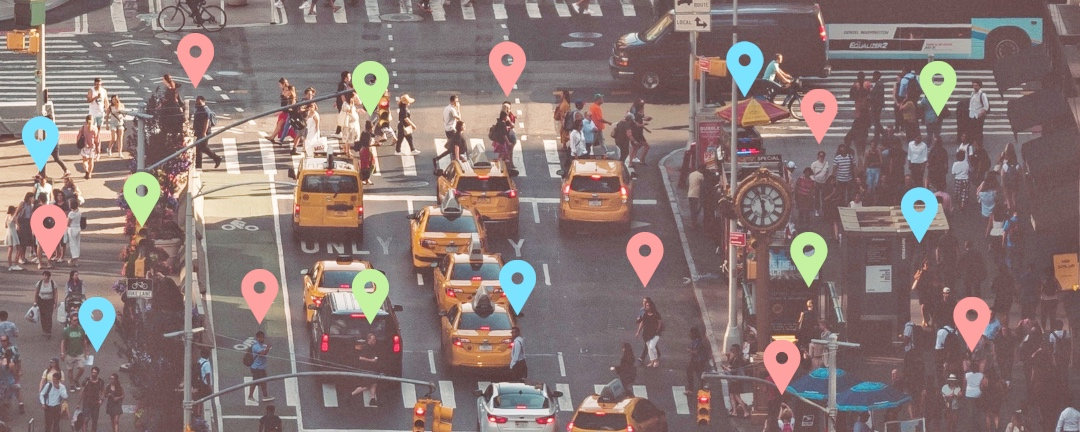
\includegraphics[width = 1\textwidth]{Images/SIR_image}\vspace{-9pt}
			\caption{\justifying Illustration of Contact-Tracing data with labeled\hspace{-1pt} \textcolor{my-blue}{\textbf{Susceptible}}, \textcolor{my-red}{\textbf{Infected}}, and \textcolor{my-green}{\textbf{Recovered}} people.}
			\label{fig:SIR-illustration}
		\end{figure}
	\end{frame}

	\begin{frame}[t]
		\frametitle{Methodology}
		\justifying
		\textcolor{titles}{\textbf{Base-SIR modeling}}  (Hernández-Orallo et al${.}$, 2020)
		
		Assuming a closed environment, we have 5 compartments and 7 events, namely
		\begin{figure}[!ht]
			\centering
			\def\svgwidth{0.85\columnwidth}\import{./Images/inkscape}{blocks.pdf_tex}
			\caption{\justifying Diagram for the 5 compartments (S, I, R, $\text{Q}_{\text{S}}$, $\text{Q}_{\text{I}}$) and 7 possible transfers.}
			\label{fig:base-SIR}
		\end{figure}
	\end{frame}

	\begin{frame}[t]
		\frametitle{Methodology}
		\justifying
		\textcolor{titles}{\textbf{Base-SIR modeling}}
		
		For each time window $t$, the interactions in the population will be represented by a \textit{network graph}; which can also be translated into a contact matrix $\text{G}(t)$.
		
		\begin{minipage}[t]{0.48\linewidth}
			\vbox to0cm{} % https://tex.stackexchange.com/questions/203082/beamer-revealing-image-in-one-minipage-moves-stuff-in-the-other-minipage
			\centering
			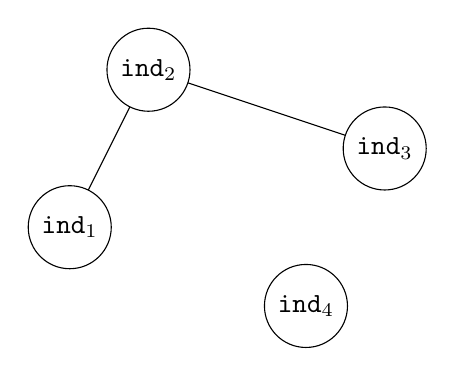
\begin{tikzpicture}
				\draw[black] (1,1) -- (2,3);
				\draw[black] (2,3) -- (5,2);
				\draw[fill=white] (1,1) circle (15pt);
				\draw[fill=white](2,3) circle (15pt);
				\draw[fill=white] (5,2) circle (15pt);
				\draw[fill=white] (4,0) circle (15pt);
				\node[] at (1,1) {$\texttt{ind}_1$};
				\node[] at (2,3) {$\texttt{ind}_2$};
				\node[] at (5,2) {$\texttt{ind}_3$};
				\node[] at (4,0) {$\texttt{ind}_4$};
			\end{tikzpicture}
		\end{minipage}\hfill \pause
		\begin{minipage}[t]{0.48\linewidth}
			\centering
			\[ \text{G}(t) = 
			\begin{bmatrix}
				0 & 1 & 0 & 0 \\
				1 & 0 & 1 & 0 \\
				0 & 1 & 0 & 0 \\
				0 & 0 & 0 & 0
			\end{bmatrix},
			\]
			\justifying
			such that $\text{G}_{ij}(t) = \text{G}_{ji}(t)$, for all pairs $(i, j)$, \hspace{-2pt}and $\text{G}_{ii}(t) = 0$, $\forall i$.
		\end{minipage}
	\end{frame}

	\begin{frame}[t]
		\frametitle{Methodology}
		\justifying
		\textcolor{titles}{\textbf{Base-SIR modeling}}
		
		Regarding the tracing data, the \textit{number of infectious contact} $\mathcal{K}_i(t)$ can be defined as follows
		\begin{align*}
			\mathcal{K}_i(t) = \sum_{j = 1}^{\text{N}}\text{G}_{ij}(t)\text{I}_j(t) ,
		\end{align*}
		where $\text{N}$ is the total number of individuals, and $\text{I}_{j}(t)$ is an indicator function for the event in which the individual $j$ can infect others.
	\end{frame}

	\begin{frame}[t]
		\frametitle{Methodology}
		\justifying
		\textcolor{titles}{\textbf{Base-SIR modeling}}
		
		Also, as a way to track back the contacts, we can define, for some $t$ and a time period $\Delta$, a function that verify whether an individual has had contact with at least one traced individual; that is, we want to define $\mathcal{C}_i(t, \Delta)$, such that 
		\[ \mathcal{C}_i(t, \Delta) = 
		\begin{cases} 
			1 & \text{if }\sum_{j = 1}^{\text{N}} \left(\max_{\tau \in [t - \Delta, t]}\text{G}_{ij}(\tau)\right)\text{D}_{j}(t) > 0 \\
			0 & \text{otherwise},
		\end{cases}
		\]
		such that $\text{D}_j(t)$ is an indicator function for the event in which the individual $j$ is infected and traced.
		
		%\pause
		%Also, let $q$ be defined as the \textit{tracing efficiency}.
	\end{frame}

	\begin{frame}[t]
		\frametitle{Methodology}
		\justifying
		%\textcolor{titles}{\textbf{Base-SIR modeling}}

		\begin{table}[!ht]
			\centering
			\footnotesize
			\begin{tabular}{c|c|l} 
				\hline
				Event & Rate Equation & Description \\
				\hline
				$\text{S}\rightarrow\text{I}$ & $(1 - \mathcal{C}_i(t, \triangle)) \cdot b \cdot \mathcal{K}_i(t)$ & Non-traced infected individuals. \\
				$\text{S}\rightarrow\text{Q}_{\text{S}}$ &  $\mathcal{C}_i(t, \triangle) \cdot (1 - b \cdot \mathcal{K}_i(t))$ & Non-infected but traced individuals. \\
				$\text{S}\rightarrow\text{Q}_{\text{I}}$ &  $\mathcal{C}_i(t, \triangle) \cdot b \cdot \mathcal{K}_i(t)$ & Infected and traced individuals. \\
				$\text{I}\rightarrow\text{Q}_{\text{I}}$ &  $\delta$ & Detection of infected individuals. \\
				$\text{Q}_{\text{S}}\rightarrow\text{S}$ &  $\tau_Q$ & End of quarantine for susceptible individuals. \\
				$\text{I}\rightarrow\text{R}$ &  $\gamma$ & Infected individuals recovered from the disease. \\
				$\text{Q}_{\text{I}}\rightarrow\text{R}$ & $\tau_Q$ & End of quarantine for infected individuals.
			\end{tabular}%
			\label{table:rate-equations}
		\end{table}
	Such that $\mathcal{K}_i(t)$ is the \textit{number of infectious contacts}, $\mathcal{C}_i(t, \triangle)$ is an indicator function for the event in which an individual has had contact with at least one traced and infected person, $b$ is the \textit{probability of transmission}, $\delta$ is the \textit{detection rate}, $1/\tau_{\text{Q}}$ is the \textit{average quarantine time}, and $\gamma$ is the \textit{recovery rate}.
	\end{frame}

	\begin{frame}[t]
		\frametitle{Methodology}
		\justifying
		\textcolor{titles}{\textbf{New spatio-temporal-SIR modeling}}
		
		As in Mahmood et al${.}$ (2021), we can incorporate the idea of \textit{temporally varying spatial risk}; meaning that, for a time windows $(t-1)$, we will collect information on the individuals that walked within a particular cell (determined by a superimposed grid over the studied region), and use such data to update their rates for the next step of an iterative process.
		
		%\pause
		
		%Also, regarding the time windows, we will define them as 4-hour interval going from 8:00 AM to 8:00 PM each day. Here, notice that, although it would ideal having close to real-time observations, windows may not be too short, since we might not observe any contacts in this case.
		
	\end{frame}

	\begin{frame}[t]
		\frametitle{Methodology}
		\justifying
		\textcolor{titles}{\textbf{New spatio-temporal-SIR modeling}}		
		\begin{figure}[!ht]
			\centering
			\def\svgwidth{\columnwidth}\import{./Images/inkscape}{diagram2.pdf_tex}
			\caption{\justifying Computed Relative Risk (\texttt{RR}) from contact-tracing data and covariates.}
			\label{fig:rr-modeling}
		\end{figure}
	\end{frame}

%	\begin{frame}[t]
%		\frametitle{Methodology}
%		\justifying
%		\textcolor{titles}{\textbf{New spatio-temporal-SIR modeling}}
%		
%		To determine how risky a particular cell is, one could compute the Standardized Contact Ratio (SCR), that is, the ratio of the observed counts of an event of interest and the expected counts of the same events. In particular, all $j$,
%		\begin{align*}
%			\text{SCR}_j = \frac{\text{Y}_j}{\text{E}_j},
%		\end{align*}
%		where $\text{Y}_j$ represents the number of contacts between one infected and one susceptible individual inside cell $j$, and $\text{E}_j$ represents the number of contacts of the same type that one would expect to observe in $j$, if population from this cell behaved in the same way as the general population. 
%	\end{frame}
%
%	\begin{frame}[t]
%		\frametitle{Methodology}
%		\justifying
%		\textcolor{titles}{\textbf{New spatio-temporal-SIR modeling}}
%		
%		More specifically, $\text{Y}_j = c^{is}_{j}$ and $\text{E}_j = (\texttt{cont}_j \cdot \theta_{\text{all}})$, such that
%		\begin{align*}
%			\theta_{\text{all}} = \frac{\sum_{\text{all} j}\text{Y}_j}{\sum_{\text{all} j}\texttt{cont}_j},
%		\end{align*}
%		where $\texttt{cont}_j = (c^{is}_{j} + c^{ii}_{j} + c^{ss}_{j})$,
%		$c^{is}_{j}$ is the number of contacts between an infected person and a susceptible one, $c^{ii}_{j}$ the number of contacts between two infected people, and $c^{ss}_{j}$ the number of contacts between two susceptible people. 
%		
%		\pause
%		
%		However, if the number of reported occurrences of the event of interest in a particular cell, say $j$, is not sufficiently large, then $\text{SCR}_j$ becomes less reliable.
%	\end{frame}

	\begin{frame}[t]
		\frametitle{Methodology}
		\justifying
		\textcolor{titles}{\textbf{New spatio-temporal-SIR modeling}}
		
		For $\text{Y}_j$ representing the number of contacts between one infected and one susceptible individual in a cell $j$ (as before), we will set 
		\begin{align}\label{eq:main-model}
			\text{Y}_j \sim \text{Poisson}(\text{E}_j\cdot\theta_j), \text{~for all~} j,
		\end{align}
		where $\log(\theta_j) = \beta_0 + \beta_1 \cdot x_{1j} + \cdots +  \beta_p \cdot x_{pj} + u_j$, such that $x_{1j}, \cdots, x_{pj}$ are covariates that affect the risk (e.g., \# of buildings) in $j$, and $u_j \overset{\text{i.i.d.}}{\sim} \text{Normal}(0, \sigma^2_{u})$. 
		
		Also, $\text{E}_j = (\texttt{cont}_j \cdot \theta_{\text{all}})$, such that
		\begin{align*}
			\theta_{\text{all}} = \frac{\sum_{\text{all} j}\text{Y}_j}{\sum_{\text{all} j}\texttt{cont}_j},
		\end{align*}
		where $\texttt{cont}_j = (c^{is}_{j} + c^{ii}_{j} + c^{ss}_{j})$.
		
		%\pause
		
		%As a \textit{remark}, notice that $\log(\theta_j)$ could have been defined in a different manner; in particular, we could have added a random effect $\nu_j$ specific to cell $j$ that models the spatial dependence between relative risks.
	\end{frame}

	\begin{frame}[t]
		\frametitle{Methodology}
		\justifying
		\textcolor{titles}{\textbf{New spatio-temporal-SIR modeling}}
		
		In Model \eqref{eq:main-model}, the Relative Risk (\texttt{RR}) $\theta_j$ quantifies whether area $j$ has higher ($\theta_j > 1$) or lower ($\theta_j  < 1$) risk than the average risk in the population.
		
		\pause
		
		Also, as we may not observe contacts in some cells, we cannot say much about whether these regions are more or less risky than the overall considered area. In this case, if $\texttt{cont}_j = 0$ for some $j$, we chose to set $\texttt{RR}_j$ to 1.
	\end{frame}

	\begin{frame}[t]
		\frametitle{Simulation}
		\justifying	
		Using the \texttt{Simulation of Urban Mobility} (SUMO) library, we simulated the movement of $1{,}000$ pedestrians in part of Valencia, Spain, for 150 days.
		
		\begin{figure}
			\centering \vspace{-16pt}
			\includegraphics[width = 0.7\textwidth]{Images/pedestrians_transp} \vspace{-22pt}
			\caption{\justifying SUMO simulated trajectories for 10 randomly selected pedestrians in the ``day 1'' in Valencia. ``\texttt{ID \#}''\hspace{-2pt} refers to the pedestrian code number in the data set.}
			\label{fig:pedestrians}
		\end{figure}\vspace{-3pt}
	\end{frame}

%	\begin{frame}[t]
%		\frametitle{Simulation}
%		\justifying	
%		
%		The region from Figure \ref{fig:pedestrians} was divided into 230 cells and, aiming at increasing the number of contacts, 23 cells (same cells with high building density) were set as \textit{high priority}.
%		\begin{figure}[!ht]
%			\centering \vspace{-8pt}
%			\includegraphics[width = 1\textwidth]{Images/buildings-contacts_transp} \vspace{-30pt}
%			\caption{\justifying 23 selected cells (left), and cells where at least one contact occurred (right). Red dots indicate the buildings.}
%			\label{fig:buildings-contacts}
%		\end{figure}
%	\end{frame}
	
	\begin{frame}[t]
		\frametitle{Implementation}
		\justifying	
		
		Based on the simulated data set, we define a model for the Relative Risks (\texttt{RR}s) for all $ j = 1, 2, \cdots, 230$, and for all time windows. In particular,
		\begin{align*}
			\text{Y}_j \sim \text{Poisson}(\text{E}_j \cdot \theta_j), \text{ for } j = 1, \cdots, 230, \text{ such that $\texttt{cont}_j \neq 0$},
		\end{align*}
		where $\log(\theta_j) = \beta_0 + \beta_1 \cdot x_{1j} + u_j$, such that $x_{1j}$ represents the number of buildings in cell $j$ and $u_j \overset{\text{i.i.d.}}{\sim} \text{Normal}(0, \sigma^2_{u})$.
	\end{frame}
	
	\begin{frame}[t]
		\frametitle{Implementation}
		\justifying	
		
		Now, to incorporate this temporally varying spatial risk into our compartment model, we will update the $\text{G}(t)$ matrix, such that $\text{G}^{\star}(t)$ at the position $(k, \ell)$ will be given by $\texttt{RR}_j$, if individuals $k$ and $\ell$ have been in contact at cell $j$ for the time-window $(t - 1)$; and $0$, if there was no contact (as before).
		
		\begin{minipage}[t]{0.48\linewidth}
			\vbox to0cm{} % https://tex.stackexchange.com/questions/203082/beamer-revealing-image-in-one-minipage-moves-stuff-in-the-other-minipage
			\centering
			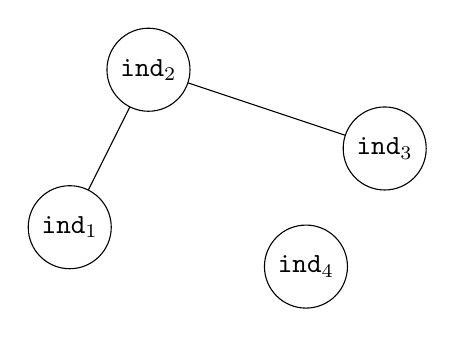
\begin{tikzpicture}
				\draw[black] (1,1) -- (2,3);
				\draw[black] (2,3) -- (5,2);
				\draw[fill=white] (1,1) circle (15pt);
				\draw[fill=white](2,3) circle (15pt);
				\draw[fill=white] (5,2) circle (15pt);
				\draw[fill=white] (4,0.5) circle (15pt);
				\node[] at (1,1) {$\texttt{ind}_1$};
				\node[] at (2,3) {$\texttt{ind}_2$};
				\node[] at (5,2) {$\texttt{ind}_3$};
				\node[] at (4,0.5) {$\texttt{ind}_4$};
			\end{tikzpicture}
		\end{minipage}\hfill
		\begin{minipage}[t]{0.48\linewidth}
			\centering
			\[ \text{G}^{\star}(t) = 
			\begin{bmatrix}
				0 & \texttt{RR}_j & 0 & 0 \\
				\texttt{RR}_j & 0 & \texttt{RR}_j & 0 \\
				0 & \texttt{RR}_j & 0 & 0 \\
				0 & 0 & 0 & 0
			\end{bmatrix},
			\]
			\justifying
		\end{minipage}
		
		%Considering such a model, we simulated the evolution of an epidemic for both ``base-SIR'' and ``new spatio-temporal-SIR'' modeling approaches. That is, for a common set of parameters (which may be disease specific; e.g., \textit{transmission rate}), we simulated the trajectories of individuals in each compartment ${}^{(1)}$ without accounting for the RR, and ${}^{(2)}$ accounting for the RR.  
	\end{frame}

	\begin{frame}[t]
		\frametitle{Results}
		\justifying	
		\textcolor{titles}{\textbf{Base-SIR model}}
		
		\begin{figure}
			\centering \vspace{-6pt}
			\includegraphics[width = 1\textwidth]{Images/fitted-base_transp} \vspace{-30pt}
			\caption{\justifying Number of individuals in each compartment (S, I, R, $\text{Q}_{\text{S}}$, $\text{Q}_{\text{I}}$) over the days using the base-SIR model. Light lines represent the 10 realizations of the simulated epidemic, and the bold line represents their average.}
			\label{fig:fitted-base}
		\end{figure}\vspace{-6pt}
	\end{frame}

	\begin{frame}[t]
		\frametitle{Results}
		\justifying	
		\textcolor{titles}{\textbf{New spatio-temporal-SIR modeling}}
		
		\begin{figure}
			\centering \vspace{-8pt}
			\includegraphics[width = 0.9\textwidth]{Images/RRs} \vspace{-10pt}
			\caption{\justifying Estimated RRs for all cells in the second window of days 1, 2, 3, and 4.}
			\label{fig:estimatedRR}
		\end{figure}\vspace{-6pt}
		
	\end{frame}


	\begin{frame}[t]
		\frametitle{``Base-SIR'' (T) and ``new spatio-temporal-SIR model'' (B) }
		\justifying	
		%\textcolor{titles}{\textbf{New spatio-temporal-SIR model}}
	
		\begin{figure}
			\centering \vspace{-6pt}
			\includegraphics[width = 0.75\textwidth]{Images/fitted-base_transp} \vspace{-30pt}
			\includegraphics[width = 0.75\textwidth]{Images/fitted-temporal_transp} \vspace{-30pt}
			%\caption{\justifying ``Base-SIR'' (top) and ``new spatio-temporal-SIR model'' (bottom) plots.}
			%\caption{\justifying Number of individuals in each compartment (S, I, R, $\text{Q}_{\text{S}}$, $\text{Q}_{\text{I}}$) over the days using the spatio-temporal-SIR model. Light lines represent the 10 realizations of the simulated epidemic, and the bold line represents their average.}
			\label{fig:fitted-temporal}
		\end{figure}\vspace{-6pt}
	\end{frame}

	\begin{frame}[t]
		\frametitle{Discussion}
		\justifying	
		\begin{enumerate}
			\item \justifying With the ``new spatio-temporal-SIR'' model, since riskier areas affect more the disease transmission, people who visit these cells are more likely to be quarantined and the peak of the simulated epidemic was reduced.\pause
			\item \justifying Having close to \textit{real-time} knowledge about risky areas in, say a city, allows politics to propose policies that will prevent individuals from walking around dangerous spots during a specific time-windows.\pause
			\item \justifying One could argue that not allowing people to go out would prevent any new cases to be observed. However, as these restrictions also impact other areas of the citizens’ lives, having frequently updated information may help politics to focus on areas that matter.\pause
			\item \justifying Contact-tracing data is difficult to obtain due to privacy issues.
		\end{enumerate}
	\end{frame}
			

	\begin{frame}[t] % allowframebreaks
		\frametitle{References}
		\justifying
		\small
		\nocite{hernandez2020evaluating}
		\nocite{mahmood2021contextual}
		\nocite{moraga2019geospatial}
		\nocite{SUMO2018}
		\bibliographystyle{ieeetr} % plain
		\bibliography{References/References}
	\end{frame}
	
\end{document}